\section{Experiments}
\label{section:experiments}

In this section, the proposed model is applied to two benchmark synthetic datasets (Pinwheel
and Two-circles) and one real-world dataset (MNIST). On one of the synthetic
datasets, one shortcoming of the model is brought to attention, but is overcome
in a semi-supervised setting. On the real-world dataset, the model's clustering
capabilities are evaluted, as well as its capacity to model complex distributions.
A technique inspired in \autocite{mixae} was employed to improve training
speed and quality of results. This consists in dividing the inputs of the softmax layer in
the variational posterior by a \q{temperature} value, $T$, which follows
an exponential decay schedule during training. This makes the
variational posterior \q{more certain} as training proceeds, while allowing all
components to be exposed to the whole data, during the initial epochs.
Moreover, it discourages components from being \q{subtrained} during the initial epochs
and, subsequently, from being prematurely discarded.

\subsection{Toy datasets}
\subsubsection{Pinwheel dataset}

This dataset is constituted by five non-linear \q{wings}. See Figure \ref{fig:pinwheel}
for the results of running the model on this dataset. As expected, the variational
posterior has learned to partition the space so as to attribute each \q{wing} to
a component of the mixture. 
\begin{figure}
\centering
  \begin{subfigure}[t]{.5\textwidth}
    \raggedleft
    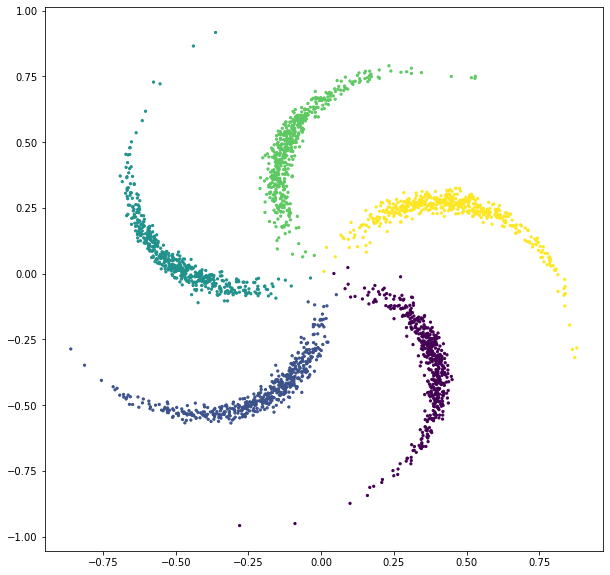
\includegraphics[width=0.6\linewidth]{figures/original_pinwheel.png}
  \end{subfigure}%
  \begin{subfigure}[t]{.5\textwidth}
    \raggedright
    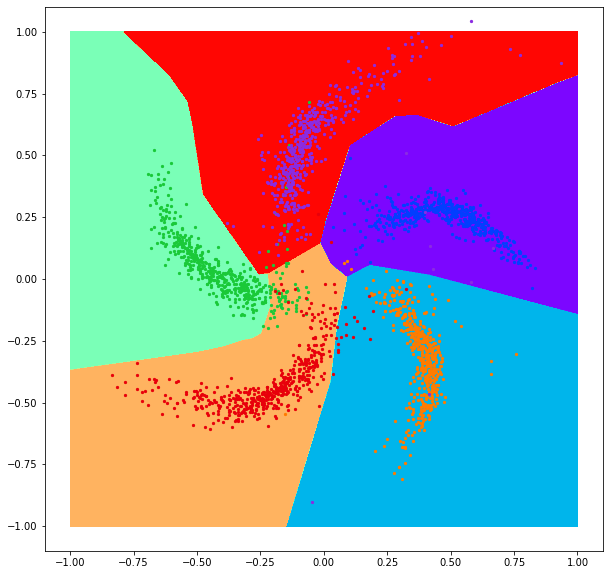
\includegraphics[width=0.6\linewidth]{figures/trained_pinwheel.png}
  \end{subfigure}
  \caption{\scriptsize (a) Original dataset (b) Samples from the learned model. Each
dot is colored according to the component it was sampled from. The background
colors denote the regions where each component has maximum probability assigned
by the variational posterior. (Note that the background colors were chosen
so as to not match the dot colors, otherwise it dots wouldn't be visible)}
  \label{fig:pinwheel}
\end{figure}

\subsubsection{Two-circles dataset}
This dataset consists of two concentric circles. The experiment on this dataset,
makes evident one shortcoming of the proposed model: the way in which the variational
posterior partitions the space is not necessarily guided by the intrisic structure
in the data (see Figure \ref{fig:twocircles}-b). In the case of the two-circles
dataset, it was found that the most common partitioning arrived at consisted
simply of a split into two half-spaces. However, in a semi-supervised setting,
this behaviour can be corrected and the model successfully learns to separate the
two circles, as shown in Figure \ref{fig:twocircles}-d). In this setting, the
model was pretrained on the labeled instances and then trained with the normal procedure.
There were 1024 labeled instances, and 64 unlabeled instances.
In this case, the model has the chance to selectively refine both the variational
posterior and each of the components. As is clearly visible in Figure
\ref{fig:twocircles}, the model struggles with learning full, closed, circles;
this is because it is unable to \q{pierce a hole} in the base distribution, due
to the nature of the transformations that are applicable. Thus, to model a circle,
the model has to learn to stretch the blob formed by the base distribution, and
\q{bend it over itself}. This difficulty is also what keeps the model from learning
a structurally interesting solution in the fully unsupervised case: it is easier
for each component to learn to distort space so as to model half of the two circles.
Moreover, the points in diametrically opposed regions of the same circle are
more dissimilar (in the geometrical sense) than points in the same region of the
two circles. Therefore, when completely uninformed by labels, the variational
posterior's layers will tend to have similar activations for points in the latter
case, and thus tend to have similar outputs for them.

\begin{figure}
\centering
  \begin{subfigure}[t]{.24\textwidth}
    \centering
    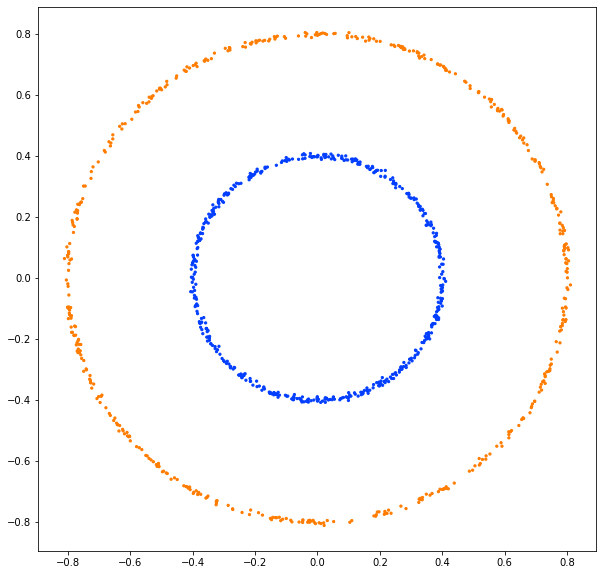
\includegraphics[width=0.9\linewidth]{figures/original_2_circles.png}
  \end{subfigure}%
  \begin{subfigure}[t]{.24\textwidth}
    \centering
    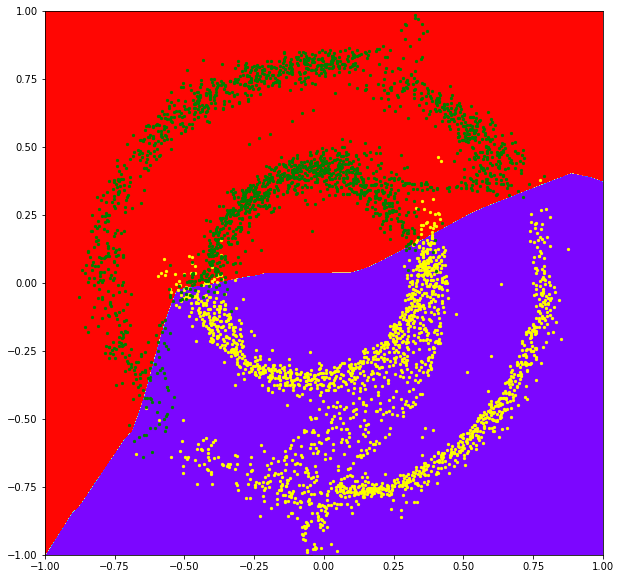
\includegraphics[width=0.9\linewidth]{figures/trained_2_circles_2.png}
  \end{subfigure}
  \begin{subfigure}[t]{.24\textwidth}
    \centering
    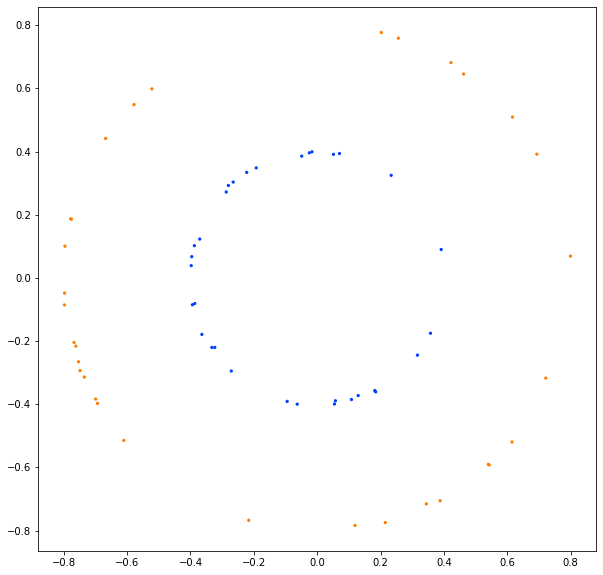
\includegraphics[width=0.9\linewidth]{figures/labeled_2_circles.png}
  \end{subfigure}%
  \begin{subfigure}[t]{.24\textwidth}
    \centering
    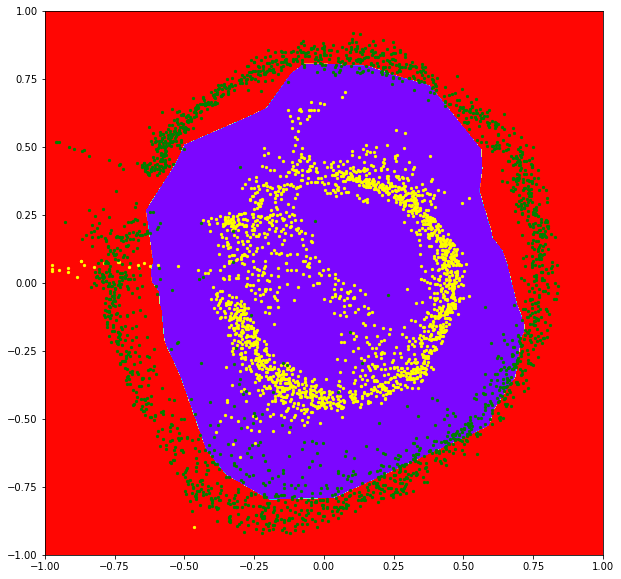
\includegraphics[width=0.9\linewidth]{figures/trained_2_circles_semisup.png}
  \end{subfigure}
  \caption{\scriptsize a) Original dataset. b) Samples from the learned model, without any labels. Coloring logic
    is the same as in Figure \ref{fig:pinwheel}. c) Labeled points used in semi-supervised scenario.
    d) Samples from the model trained in the semi-supervised scenario.}
  \label{fig:twocircles}
\end{figure}

\subsection{Real-world dataset}
In this subsection, the proposed model is evaluated on the well-known MNIST
dataset \autocite{MNIST}. For this experiment, only the images corresponding to the digits
from 0 to 4 were considered. In Figure \ref{fig:mnist_samples}, samples from the
components obtained after training can be seen. Moreover, a normalized
contingency table is presented, where the performance of the variational posterior
as a clustering function can be assessed. Note that the cluster indices induced
by the model have no semantic meaning.
\begin{figure}
\begin{floatrow}
\floatbox{figure}[.48\textwidth][\FBheight][t]{%
  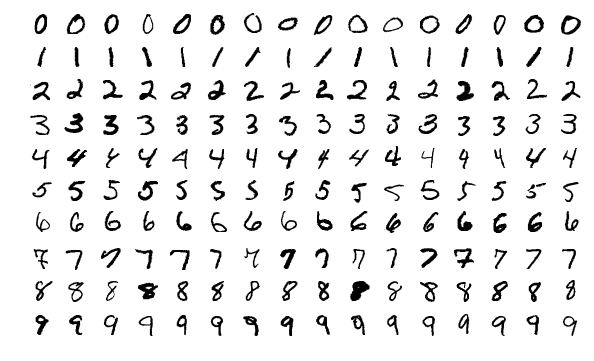
\includegraphics[width=0.90\linewidth]{figures/trained_mnist.png}%
}{%
  \caption{\scriptsize Samples from the fitted mixture components. Each row is sampled from the same component}%
  \label{fig:mnist_samples}%
}
\floatbox{table}[.48\textwidth][\FBheight][t]{%
\setlength\tabcolsep{1.3pt}
\begin{tabular}{c| *{5}{S[table-auto-round, table-format=-1.2]}}
 &         0 &         1 &         2 &         3 &         4 \\
\midrule
0    &  0.000602 &  0.012432 &  0.002807 &  0.982555 &  0.001604 \\
1    &  0.002139 &  0.020146 &  0.977001 &  0.000178 &  0.000535 \\
2    &  0.000802 &  0.952276 &  0.011630 &  0.007219 &  0.028073 \\
3    &  0.001558 &  0.479455 &  0.300682 &  0.004284 &  0.214021 \\
4    &  0.646166 &  0.347273 &  0.005125 &  0.001435 &  0.000000 \\
\bottomrule
\end{tabular}
}{%
\caption{\scriptsize Normalized contingency table for the clustering induced by the model.
Rounded to two decimal places. Rows: true label. Columns: cluster index.}%
\label{table:contingency}%
}
\end{floatrow}
\end{figure}%
%\begin{figure}[!htb]
%  \centering
%  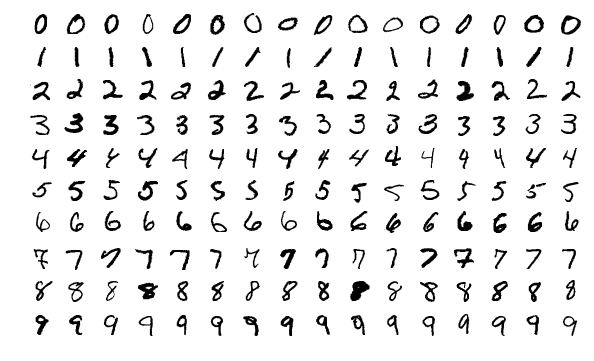
\includegraphics[width=0.60\linewidth]{figures/trained_mnist.png}
%  \caption{Samples from the fitted mixture components. Each row is sampled
%  from the same component}
%  \label{fig:mnist_samples}
%\end{figure}
%
%\begin{table}[h]
%\centering
%\begin{tabular}{cccccc}
%\toprule
%\diagbox[trim=lr]{True\\label}{Cluster\\index} &         0 &         1 &         2 &         3 &         4 \\
%\midrule
%0    &  0.000602 &  0.012432 &  0.002807 &  \textbf{0.982555} &  0.001604 \\
%1    &  0.002139 &  0.020146 &  \textbf{0.977001} &  0.000178 &  0.000535 \\
%2    &  0.000802 &  \textbf{0.952276} &  0.011630 &  0.007219 &  0.028073 \\
%3    &  0.001558 &  \textbf{0.479455} &  0.300682 &  0.004284 &  0.214021 \\
%4    &  \textbf{0.646166} &  0.347273 &  0.005125 &  0.001435 &  0.000000 \\
%\bottomrule
%\end{tabular}
%\caption{Normalized contingency table for the clustering induced by the model}
%\label{table:contingency}
%\end{table}
From Table \ref{table:contingency} and Figure \ref{fig:mnist_samples} it is possible
to see that although there is some confusion, the model successfully clusters
the MNIST digits.
